% TaskSAT: Scheduling and Verifying Task Networks with SMT
% Klaus Havelund - 2026 - 20 minutes

\documentclass{beamer}

\title{\tasksat{}\\[0.1cm]{\large Scheduling and Verifying Task Networks with SMT}}

\author{{\bf Klaus Havelund}\\
Jet Propulsion Laboratory\\
California Institute of Technology\\[0.35cm]

\includegraphics[width=4.2cm]{figures/jpl-logo.png}}

\date[]{JPL --- 2026}

\mode<presentation>
{
\usetheme{Madrid}
\setbeamercovered{transparent=5}
\setbeamertemplate{navigation symbols}{}
}

\usepackage[T1]{fontenc}   % so < > ~ in \ttfamily render correctly
\usepackage{amsmath,amssymb}
\usepackage{graphicx}
\usepackage{xcolor}
\usepackage{booktabs}
\usepackage{listings}
\usepackage{tikz}
\usetikzlibrary{arrows.meta,positioning,shapes.geometric,calc}

\definecolor{codegreen}{rgb}{0,0.6,0}
\definecolor{tncolor}{rgb}{0.10,0.35,0.75}
\definecolor{okcol}{rgb}{0.13,0.55,0.13}
\definecolor{badcol}{rgb}{0.75,0.10,0.10}

\newcommand{\tasksat}{\textsf{TaskSAT}}
\newcommand{\mexec}{\textsf{MEXEC}}
\newcommand{\zthree}{\textsf{Z3}}
\newcommand{\holds}{{\color{okcol}\bf HOLDS}}
\newcommand{\violated}{{\color{badcol}\bf VIOLATED}}

\lstdefinelanguage{tasknetdsl}{
    keywords={tasknet, end, timelines, atomic, state, cumulative, bounds, rate,
              taskdef, task, optional, request, pre, inv, maint, post, in, impacts,
              duration, duration_range, start_range, end_range, after, containedin,
              constraints, properties, prop, not, and, or, implies, always,
              eventually, until, since, active, initial, final, within, invariant,
              compositional, mutex, param},
    morecomment=[l]{//},
    morecomment=[l]{\#},
    commentstyle=\color{codegreen},
    keywordstyle=\color{tncolor}\bfseries,
    basicstyle=\ttfamily\scriptsize,
    backgroundcolor=\color{gray!6},
    frame=single,
    rulecolor=\color{black!30},
    keepspaces=true,
    showstringspaces=false,
    tabsize=2,
    aboveskip=4pt,
    belowskip=4pt,
}

\lstdefinestyle{shell}{
    language={},
    basicstyle=\ttfamily\scriptsize,
    backgroundcolor=\color{black!4},
    frame=single,
    rulecolor=\color{black!30},
    keepspaces=true,
    showstringspaces=false,
    aboveskip=4pt,
    belowskip=4pt,
}

\lstset{language=tasknetdsl}
\newcommand{\itn}{\lstinline[language=tasknetdsl,basicstyle=\ttfamily\small,backgroundcolor={},frame=none]}


\setbeamertemplate{footline}{%
  \leavevmode%
  \hbox{%
    \begin{beamercolorbox}[wd=\paperwidth,ht=1.6ex,dp=0.2ex,leftskip=0.6em,rightskip=0.6em]{author in head/foot}%
      \usebeamerfont{author in head/foot}%
      \fontsize{5}{5}\selectfont \copyright 2026.
      All rights reserved. This document has been reviewed and the information being released does not contain export controlled technical data%
      \hfill%
      \fontsize{5}{5}\selectfont \insertframenumber/\inserttotalframenumber%
    \end{beamercolorbox}%
  }%
}

\begin{document}

\begin{frame}
  \titlepage
\end{frame}

%----------------------------------------
\begin{frame}
  \frametitle{The setting: \mexec{}} \small

\begin{columns}[c]
\begin{column}{0.52\textwidth}
\centering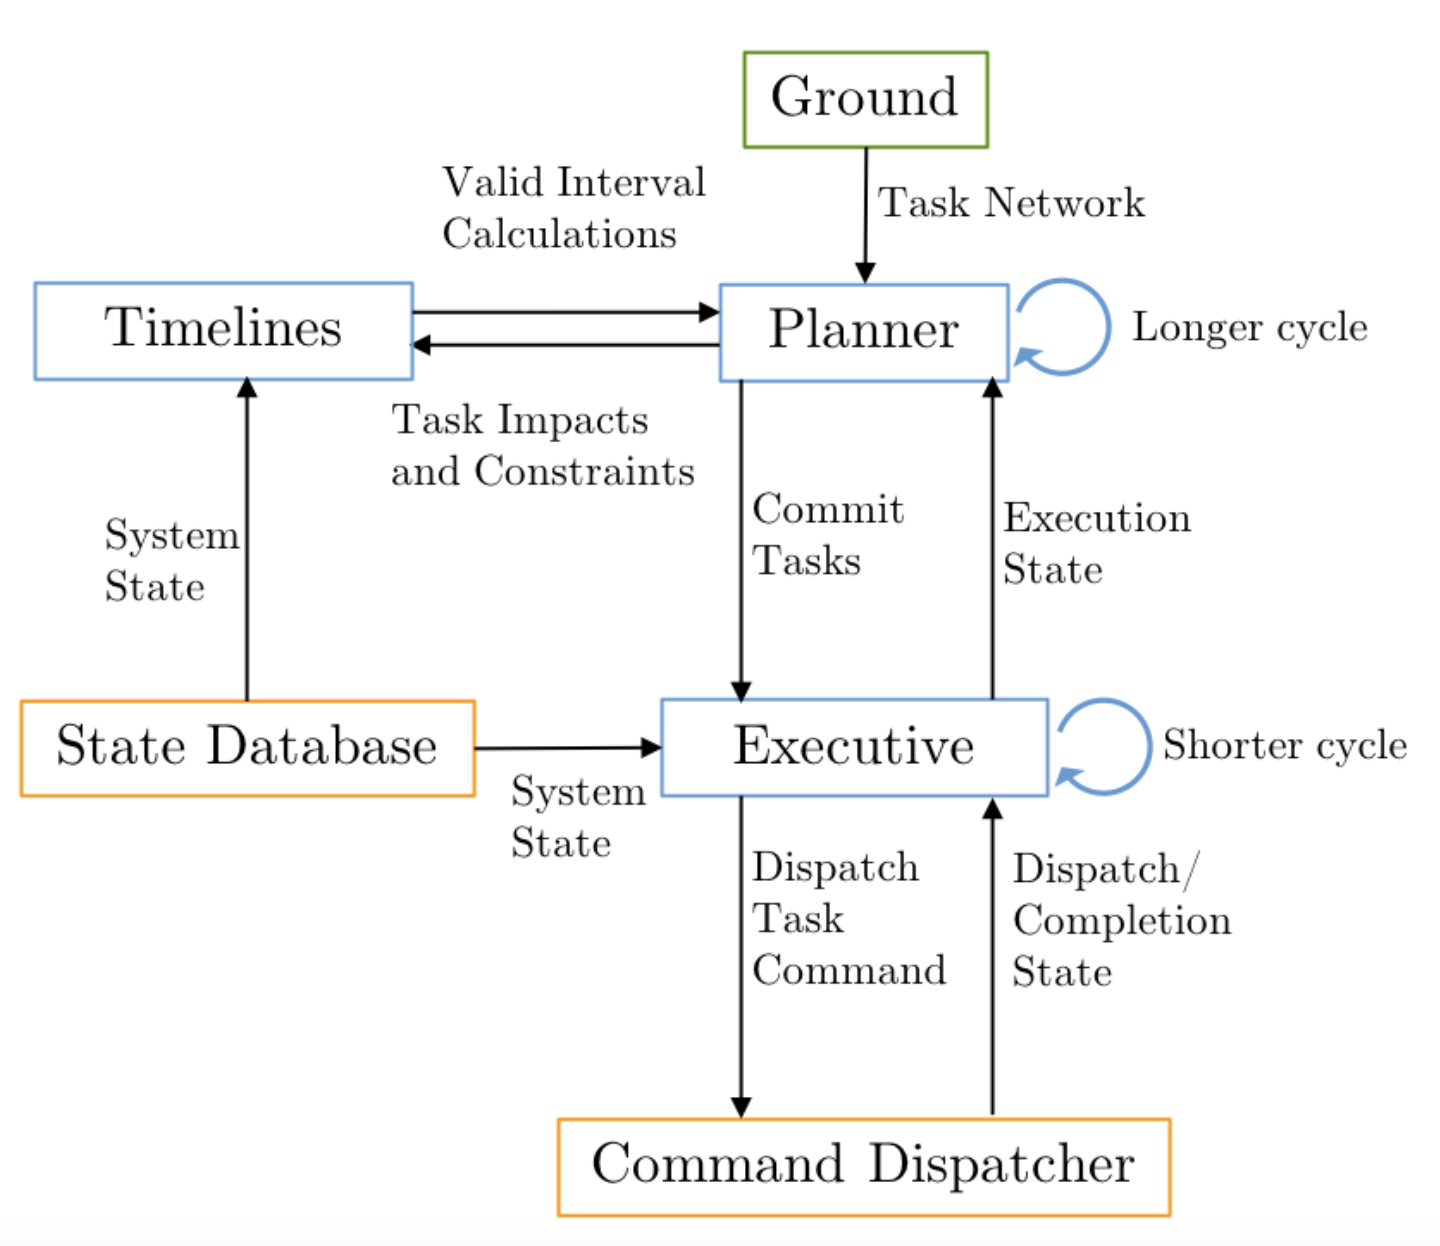
\includegraphics[width=\textwidth]{figures/mexec.png}
\end{column}
\begin{column}{0.46\textwidth}
JPL's onboard planner and executive. Ground uplinks a {\bf task network}: tasks,
the {\bf timelines} they read and write, and the constraints between them.

\vspace{0.3cm}
\mexec{} schedules it onboard and repairs the plan as it executes.

\pause
\vspace{0.3cm}
{\bf The question:} before we uplink a task network, can we know that it can be
scheduled at all, and that every schedule it admits is safe?
\end{column}
\end{columns}

\end{frame}

%----------------------------------------
\begin{frame}
  \frametitle{\tasksat{}} \small

A DSL for task networks, as close as we could get to \mexec{}'s concepts and
semantics, plus temporal logic. Solved with \zthree{}.

\vspace{0.3cm}
{\centering\scriptsize
\setlength{\tabcolsep}{4pt}
\renewcommand{\arraystretch}{1.3}
\begin{tabular}{llc}
\toprule
{\bf Question} & & {\bf Form} \\
\midrule
Validity      & Is there any schedule? (the planning problem) & $\exists i\, \exists s\, .\ \mathit{valid}(i,s)$ \\
Properties    & Is every schedule safe?                         & $\forall i\, \forall s\, .\ \mathit{valid}(i,s) \Rightarrow \varphi$ \\
\pause
Realizability & Is there a schedule from {\em every} initial state? & $\forall i\, \exists s\, .\ \mathit{valid}(i,s)$ \\
Compositional & Does it hold for {\em any} number of repetitions?  & $\{P\}\,S\,\{P\} \Rightarrow \forall N.\{P\}\,S^N\{P\}$ \\
\bottomrule
\end{tabular}\par}

\vspace{0.3cm}
$i$ is an initial state, $s$ a schedule.

\end{frame}

%----------------------------------------
\begin{frame}
  \frametitle{The pipeline} \small

{\centering
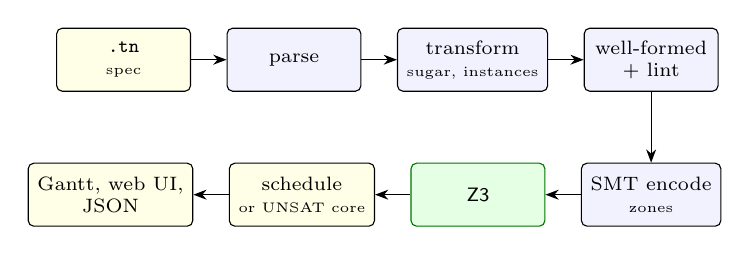
\begin{tikzpicture}[
  font=\scriptsize, >=Stealth, node distance=0.45cm,
  b/.style={draw, rounded corners=2pt, align=center, minimum height=0.8cm,
            minimum width=1.7cm, fill=blue!5},
  zz/.style={b, fill=green!10, draw=green!45!black},
  o/.style={b, fill=yellow!10}
]
  \node[o] (tn) {\tt .tn\\{\tiny spec}};
  \node[b, right=of tn]  (p) {parse};
  \node[b, right=of p]   (t) {transform\\{\tiny sugar, instances}};
  \node[b, right=of t]   (w) {well-formed\\+ lint};
  \node[b, below=0.9cm of w] (e) {SMT encode\\{\tiny zones}};
  \node[zz, left=of e]    (s) {\zthree{}};
  \node[o, left=of s]    (r) {schedule\\{\tiny or UNSAT core}};
  \node[o, left=of r]    (v) {Gantt, web UI,\\JSON};
  \draw[->] (tn) -- (p); \draw[->] (p) -- (t); \draw[->] (t) -- (w);
  \draw[->] (w) -- (e);  \draw[->] (e) -- (s); \draw[->] (s) -- (r); \draw[->] (r) -- (v);
\end{tikzpicture}\par}

\vspace{0.5cm}
\begin{itemize}
\item Much of the language is {\bf sugar}: task ranges, sessions, mutex, auto-instantiation
      are all flattened before encoding.
\item The encoding is {\bf quantifier-free}: one formula, one solver call per question.
\item Python, PLY, \zthree{}, Flask. Open source: {\tt github.com/nasa-jpl/tasksat}
\end{itemize}

\end{frame}
          %  3 min   MEXEC, the four questions, the pipeline
%----------------------------------------
\begin{frame}[fragile]
  \frametitle{A rover: timelines} \small

\begin{lstlisting}[basicstyle=\ttfamily\tiny]
tasknet Rover2 {
  end = 400;

  timelines {
    arm         : atomic = 0;
    location    : state(home, target) = home;
    data        : cumulative [0.0, 50.0]  bounds [0.0, 100.0] = 0.0;
    battery     : rate       [10.0, 100.0] bounds [0.0, 100.0] = 60.0;
    temperature : rate       [5.0, 40.0]  bounds [0.0, 100.0] = 10.0;
  }
  ...
}
\end{lstlisting}

\vspace{0.2cm}
\begin{itemize}
\item {\bf atomic}: a $[0,1]$ claim, for mutual exclusion.
\item {\bf state}: an enumeration.
\item {\bf cumulative}: a number, changed in steps.
\item {\bf rate}: a number with a rate of change: a battery, a temperature.
\item The first interval must hold at all times. The {\bf bounds} clamp.
\end{itemize}

\end{frame}

%----------------------------------------
\begin{frame}[fragile]
  \frametitle{A rover: tasks} \small

\begin{columns}[T]
\begin{column}{0.49\textwidth}
\begin{lstlisting}[basicstyle=\ttfamily\tiny]
taskdef drive_def {
  pre {
    battery in [60.0, 100.0];
    temperature in [10.0, 40.0];
  }
  impacts {
    maint { battery -~ 1.5; }
    post  { location = target; }
  }
}

task drive : drive_def {
  start_range    [100, 120];
  end_range      [130, 160];
  duration_range [30, 40];
}
\end{lstlisting}
\end{column}
\begin{column}{0.49\textwidth}
\begin{lstlisting}[basicstyle=\ttfamily\tiny]
task collect {
  duration_range [20, 30];
  pre {
    location = target;
    battery in [60.0, 100.0];
    arm = 0;
  }
  impacts {
    maint { arm += 1;
            battery -~ 0.5; }
    post  { data += 40.0; }
  }
}

optional task charge : charge_def {
  duration_range [60, 70];
}
\end{lstlisting}
\end{column}
\end{columns}

\vspace{0.1cm}
{\tt -\~{}} / {\tt +\~{}} change a {\bf rate}; {\tt +=} and {\tt =} change a {\bf value}.
An {\bf optional} task is scheduled only if it is needed.

\end{frame}

%----------------------------------------
\begin{frame}
  \frametitle{When impacts happen} \small

\begin{columns}[c]
\begin{column}{0.42\textwidth}
\centering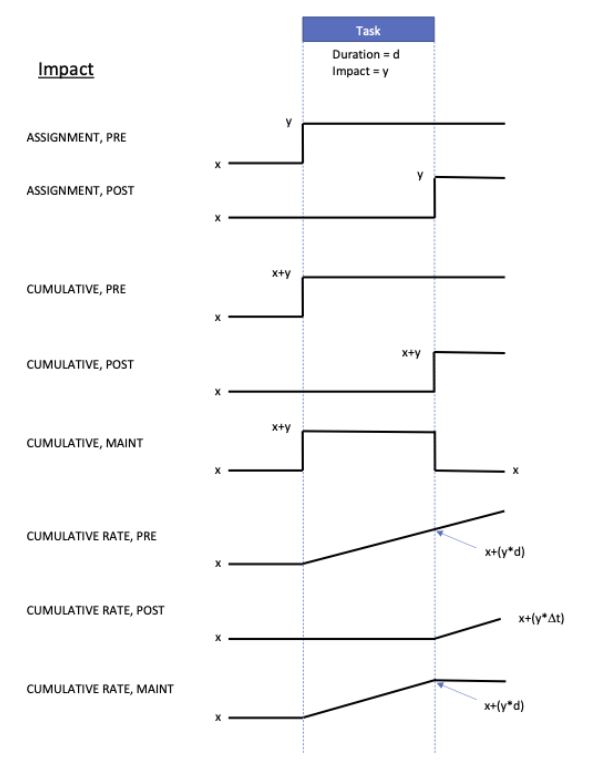
\includegraphics[height=0.78\textheight]{figures/impacts.png}
\end{column}
\begin{column}{0.56\textwidth}
\begin{itemize}
\item {\bf pre}: at the start, and stays.
\item {\bf post}: at the end, and stays.
\item {\bf maint}: at the start, undone at the end.
\end{itemize}

\vspace{0.3cm}
A task's own {\tt pre} sees the state {\em before} its impacts: {\tt collect} checks
{\tt arm = 0}, then runs with {\tt arm = 1}.

\vspace{0.3cm}
These are \mexec{}'s semantics, as best we understand them.
\end{column}
\end{columns}

\end{frame}

%----------------------------------------
\begin{frame}[fragile]
  \frametitle{Constraints and properties} \small

\begin{lstlisting}[basicstyle=\ttfamily\tiny]
constraints {
  prop not_charge_drive:   always not (active(charge) and active(drive));
  prop not_charge_collect: always not (active(charge) and active(collect));
  prop temperature10:      always temperature >= 10;
}
\end{lstlisting}

{\bf Constraints} restrict which schedules are valid.

\pause
\vspace{0.3cm}

\begin{lstlisting}[basicstyle=\ttfamily\tiny]
properties {
  prop target_reached: eventually (location = target and data >= 30);
  prop drive_charge:   always (active(drive) -> eventually active(charge));
  prop temperature:    always temperature >= 10;
}
\end{lstlisting}

{\bf Properties} are proved for {\em all} valid schedules, or refuted with a counterexample.

\vspace{0.2cm}
Past-time operators too: {\tt since}, {\tt once}, {\tt sofar}.

\end{frame}

%----------------------------------------
\begin{frame}
  \frametitle{The schedule} \small

\vspace{-0.15cm}
{\centering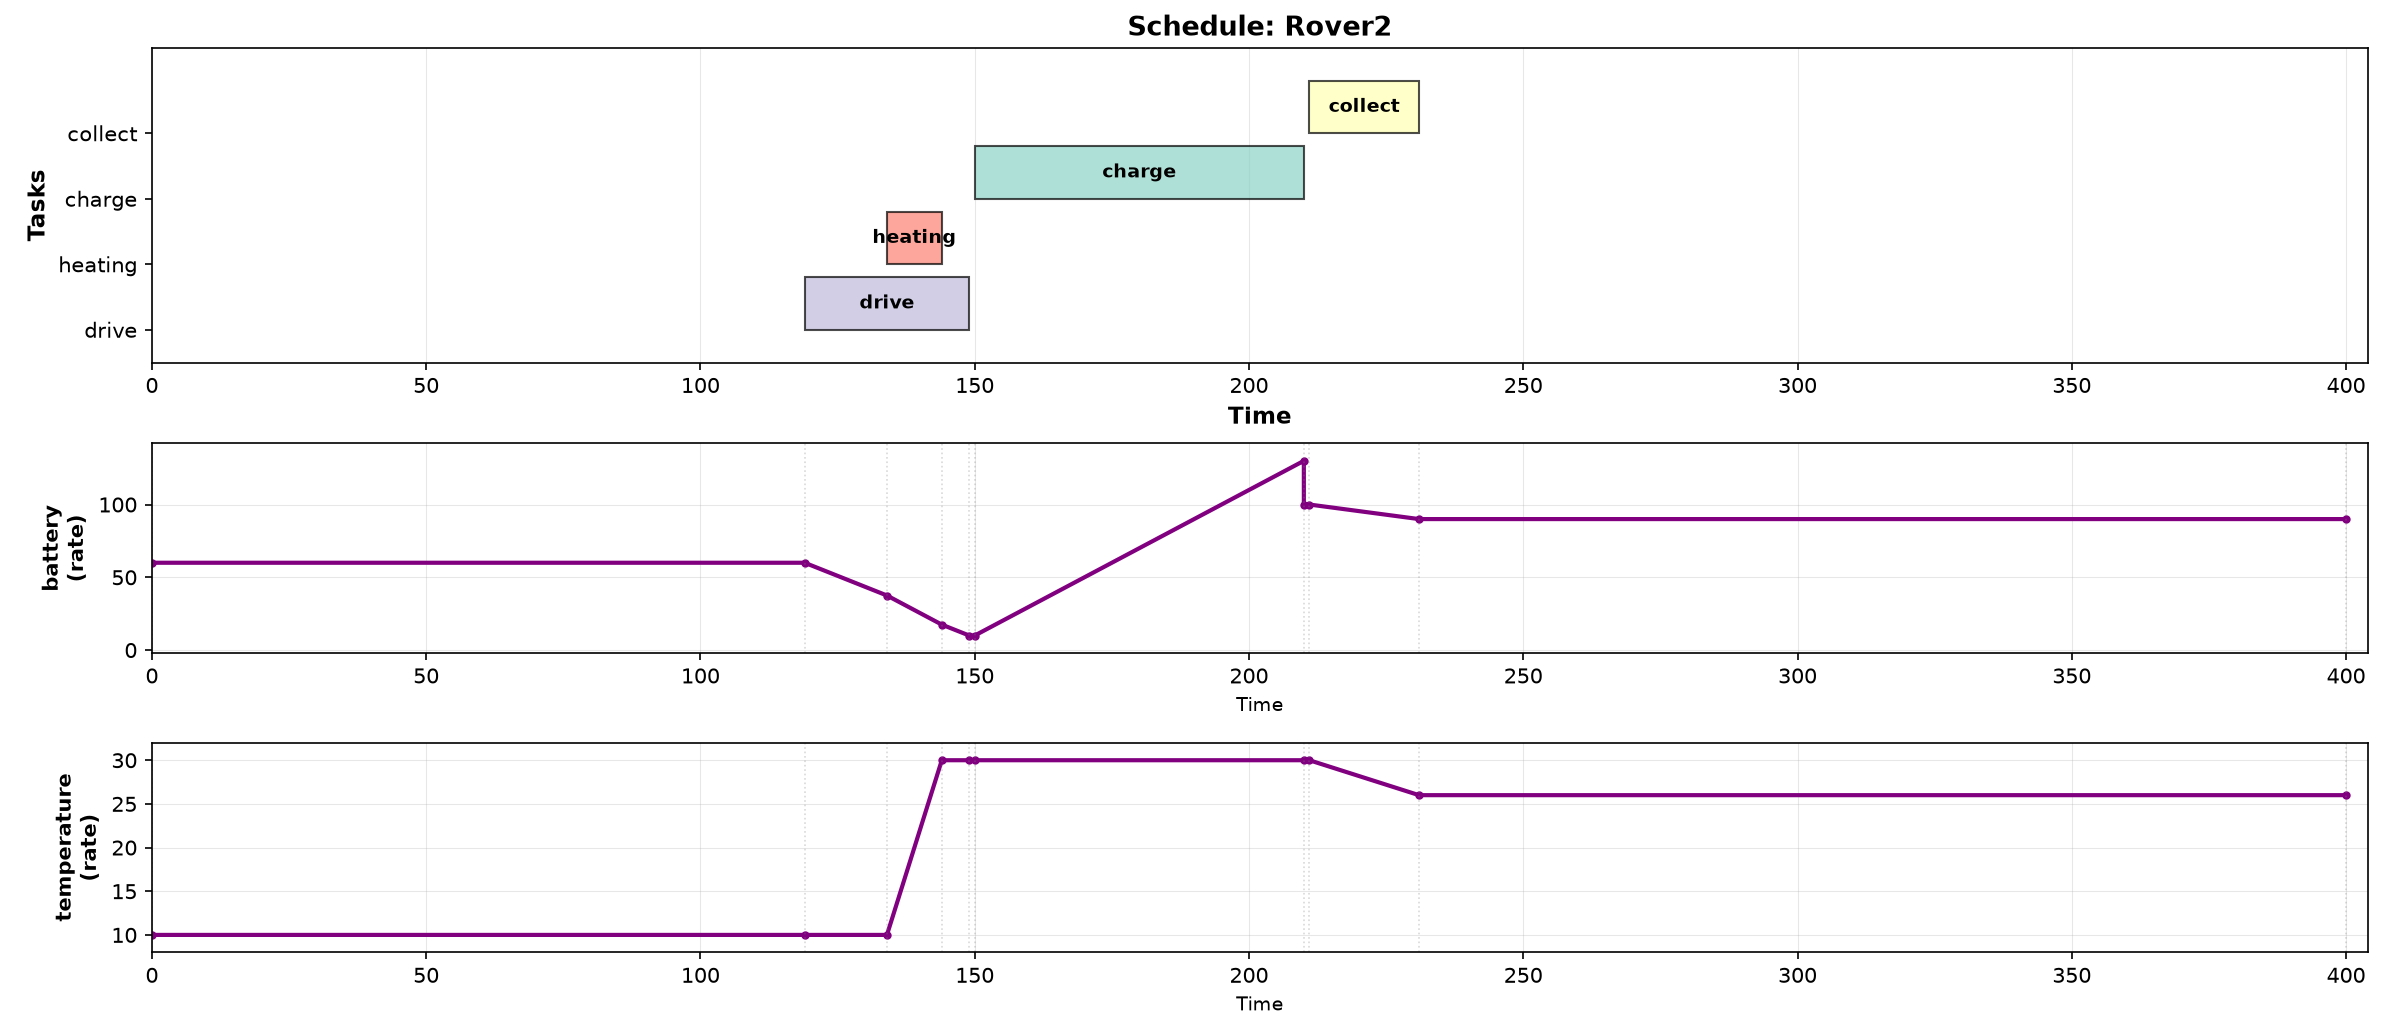
\includegraphics[width=\textwidth]{figures/rover2-timeline.png}\par}

\vspace{0.1cm}
Drive first, from the 60\% we start with, down to 10\%. Then charge to 100\% and collect.
{\tt heating} keeps the temperature up.
Charging first would waste most of it: the battery is full after 20 of its $\ge 60$ time units.

\end{frame}

%----------------------------------------
\begin{frame}
  \frametitle{The properties} \small

\vspace{-0.1cm}
{\centering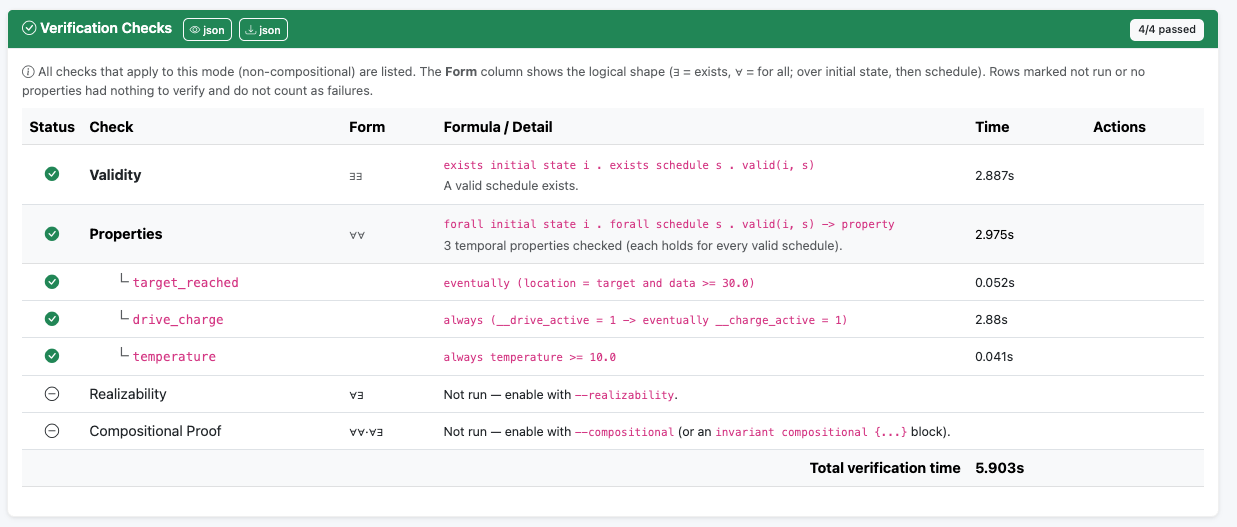
\includegraphics[width=\textwidth]{figures/rover2-results.png}\par}

\vspace{0.2cm}
Validity and the three properties, each with its logical form. 6 seconds in total.

\end{frame}

%----------------------------------------
\begin{frame}[fragile]
  \frametitle{When there is no schedule} \small

Ask for {\tt charge} to come first:

\begin{lstlisting}
task drive : drive_def {
  ...
  after charge;
}
\end{lstlisting}

\begin{lstlisting}[style=shell,basicstyle=\ttfamily\tiny]
=== Phase 1: Validity Check (EE) ===
UNSAT CORE (126 conflicting constraints)
  ...
  1. task_start_range: task 'drive' start must be in [100,120]
  2. task_end_range: task 'drive' end must be in [130,160]
  3. task_duration_range: task 'drive' duration must be in [30,40]
  4. dependency_after: 'drive' after 'charge'
  ...
  6. task_duration_range: task 'charge' duration must be in [60,70]
\end{lstlisting}

Charging first fills the battery (clamped at 100), {\tt drive} takes it to at most 55, and
{\tt collect} needs 60. There is only one {\tt charge}. Every constraint is labelled, so the
core reads back as the spec.

\end{frame}
       %  6 min   the Rover example, schedule, UNSAT
%----------------------------------------
\begin{frame}
  \frametitle{Zones: time is cut at task boundaries} \small

{\centering
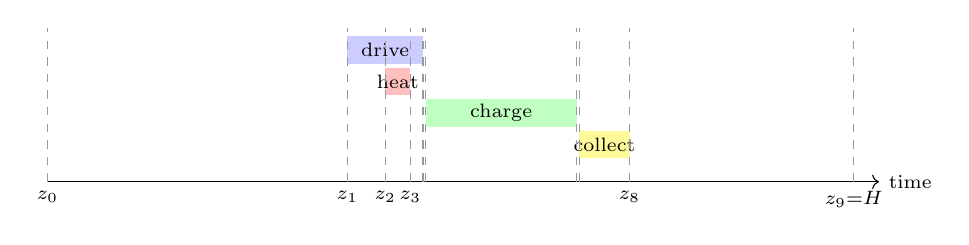
\begin{tikzpicture}[x=0.032cm, y=0.5cm, font=\scriptsize]
  % tasks
  \fill[blue!20]   (119,3) rectangle (149,3.7); \node at (134,3.35) {drive};
  \fill[red!25]    (134,2.2) rectangle (144,2.9); \node at (139,2.55) {heat};
  \fill[green!25]  (150,1.4) rectangle (210,2.1); \node at (180,1.75) {charge};
  \fill[yellow!40] (211,0.6) rectangle (231,1.3); \node at (221,0.95) {collect};
  % axis
  \draw[->] (0,0) -- (330,0) node[right] {time};
  \foreach \z/\l in {0/z_0,119/z_1,134/z_2,144/z_3,149/,150/,210/,211/,231/z_8}
    { \draw[dashed, black!40] (\z,0) -- (\z,3.9); \node[below] at (\z,0) {$\l$}; }
  \node[below] at (320,0) {$z_9{=}H$};
  \draw[dashed, black!40] (320,0) -- (320,3.9);
\end{tikzpicture}\par}

\vspace{0.3cm}
\begin{itemize}
\item Zone boundaries $z_0 < z_1 < \dots$ are SMT variables; every task start and end
      {\bf is} a zone boundary, and vice versa. Nothing changes inside a zone.
\item Each timeline gets {\bf one value per zone}, so the formula is $O(\#\mathit{tasks} \times \#\mathit{timelines})$,
      independent of the horizon.
\item Impacts are case splits on which boundary a task's start or end equals.
\end{itemize}

\end{frame}

%----------------------------------------
\begin{frame}
  \frametitle{The one nonlinear term} \small

A rate timeline $\ell$ has a value $v[j]$ and a rate $\rho[j]$ per zone:

\[
v[j{+}1] \;=\; \mathit{clamp}\big(\,v[j] \;+\; \underbrace{\rho[j] \cdot (z_{j+1} - z_j)}_{\text{rate} \,\times\, \text{zone width}} \;+\; \Delta[j]\,\big)
\]

\vspace{0.2cm}
Both factors are unknowns: the only product of two variables in the encoding.

\pause
\vspace{0.4cm}
\begin{itemize}
\item It is what makes batteries hard. A network where many tasks drain one battery
      couples them all through these products.
\item It is also an opportunity: {\bf fix the times, and the formula becomes linear}.
      Realizability exploits exactly this.
\end{itemize}

\end{frame}

%----------------------------------------
\begin{frame}
  \frametitle{Checking a property} \small

Temporal formulas are unfolded over the zones, e.g.
\[
\mathtt{always}\ \varphi \;=\; \bigwedge_j \varphi[j]
\qquad
\mathtt{eventually}\ \varphi \;=\; \bigvee_j \varphi[j]
\]

\vspace{0.2cm}
To prove $\varphi$ for {\em all} schedules, ask \zthree{} for a schedule violating it:

\[
\exists i\, \exists s\, .\ \mathit{valid}(i,s) \wedge \neg\varphi(s)
\]

\vspace{0.2cm}
\begin{itemize}
\item UNSAT: $\varphi$ \holds{}, for every schedule.
\item SAT: \violated{}, and the model is the counterexample schedule.
\end{itemize}

\vspace{0.2cm}
Same idea for {\tt final \{ ... \}}: the state at the end of every schedule.

\end{frame}
       %  3 min   zones, the one nonlinear term, properties
%----------------------------------------
\begin{frame}[fragile]
  \frametitle{Realizability: the vacuity trap} \small

\begin{lstlisting}
initial { battery in [0.0, 59.0]; }

task work {
  start_range [10, 10];  duration 20;
  pre     { battery in [30.0, 100.0]; }
  impacts { post { battery += 20.0; } }
}
\end{lstlisting}

\begin{itemize}
\item {\bf Validity} passes: \zthree{} picks a battery $\ge 30$.
\item {\bf Properties} are vacuously true for battery $< 30$: there are no schedules to violate them.
\end{itemize}

\pause
\vspace{0.1cm}
$\forall i\, \exists s$ finds the problem:

\begin{lstlisting}[style=shell]
=== Phase 3: Realizability Check (AE) ===
  [iter 1] trying initial state: battery = 0
  -> VIOLATED!
  Initial state with no valid schedule:
    battery = 0
\end{lstlisting}

\end{frame}

%----------------------------------------
\begin{frame}
  \frametitle{Realizability by CEGIS} \small

$\forall\exists$ over nonlinear arithmetic is too hard to hand to \zthree{} directly. Instead:

\vspace{0.2cm}
{\centering
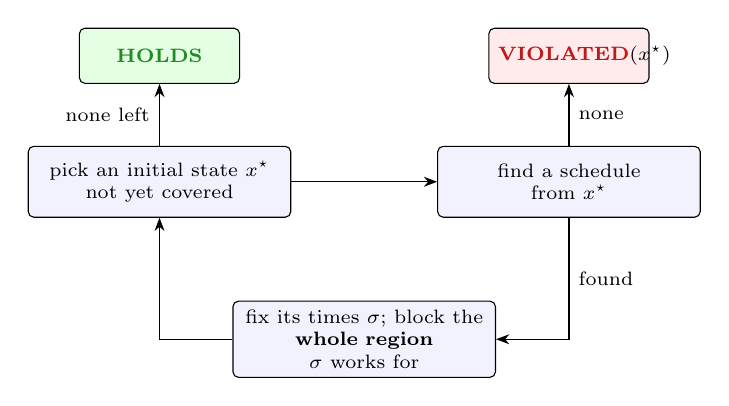
\begin{tikzpicture}[font=\scriptsize, >=Stealth,
  b/.style={draw, rounded corners=2pt, align=center, minimum height=0.9cm, text width=3.1cm, fill=blue!5},
  r/.style={draw, rounded corners=2pt, align=center, minimum height=0.7cm, text width=1.8cm}]
  \node[b] (pick) at (0,0) {pick an initial state $x^\star$\\not yet covered};
  \node[b] (solve) at (5.2,0) {find a schedule\\from $x^\star$};
  \node[b] (block) at (2.6,-2.0) {fix its times $\sigma$; block the\\{\bf whole region} $\sigma$ works for};
  \node[r, fill=green!10] (h) at (0,1.6) {\holds{}};
  \node[r, fill=red!8]    (v) at (5.2,1.6) {\violated{}($x^\star$)};
  \draw[->] (pick) -- (solve);
  \draw[->] (pick) -- node[left] {none left} (h);
  \draw[->] (solve) -- node[right] {none} (v);
  \draw[->] (solve) |- node[right, pos=0.25] {found} (block);
  \draw[->] (block) -| (pick);
\end{tikzpicture}\par}

\vspace{0.3cm}
\begin{itemize}
\item With the times fixed, the region is a {\bf linear} formula in $x$: exact, not sampled.
\item One schedule typically covers a large region, so few iterations are needed.
\end{itemize}

\end{frame}

%----------------------------------------
\begin{frame}[fragile]
  \frametitle{Compositional: verify once, repeat for free} \small

Missions repeat: drive, localize, downlink, \dots{} 200 times. The solve grows super-linearly with $N$.

\begin{lstlisting}[basicstyle=\ttfamily\tiny]
taskdef Cycle {                        // a session
  task activate   : Activate;
  task deactivate : Deactivate { after activate; }
}
invariant compositional { mode = idle; }   // P

task cycle1  : Cycle;
task cycle2  : Cycle { after cycle1; }   ...
task cycle20 : Cycle { after cycle19; }
\end{lstlisting}

\pause
Project to {\bf one} session $S$ and prove $\{P\}\,S\,\{P\}$ with {\bf two} checks:

\begin{itemize}
\item {\bf Safety} ($\forall\forall$): every schedule from $P$ ends in $P$.
\item {\bf Realizability} ($\forall\exists$): from every state in $P$, {\em some} schedule ends in $P$.
\end{itemize}

Safety alone is the vacuity trap again. Both together give $\forall N.\ \{P\}\,S^N\{P\}$.

\begin{lstlisting}[style=shell,basicstyle=\ttfamily\tiny]
=== Compositional Proof: {P}S{P} => forall N {P}S^N{P} ===
  -> HOLDS (safety=holds, realizability=holds)        -- 0.05 s, for any N
\end{lstlisting}

\end{frame}

%----------------------------------------
\begin{frame}
  \frametitle{Compositional: the fine print} \small

\begin{itemize}
\item {\bf Uniformity is enforced.} All session instances must be interchangeable;
      otherwise a $P$-preserving session followed by a $P$-breaking one would give a false \holds{}.
      Heterogeneous networks are refused.
\item {\bf No gap drift is assumed} between sessions (a battery draining while idle).
\end{itemize}

\pause
\vspace{0.3cm}
{\bf On a real \mexec{} network} (199 waypoints):

\begin{itemize}
\item The full solve does not finish. The cost is the single shared {\bf battery rate timeline},
      not symmetry and not the number of zones.
\item As flown, there is no repeating unit: driving and downlink run on independent clocks.
\item A faithful re-model with one repeating mission cycle \holds{} in 34 seconds, independent of $N$.
\end{itemize}

\vspace{0.2cm}
The method works once you {\bf supply} a repeating unit. Finding one is modelling, not solving.

\end{frame}

%----------------------------------------
\begin{frame}
  \frametitle{Lint: cheap explanations before the solve} \small

Static checks that run on every verification, in time linear in the spec. They never
block a run: the solver stays the authority.

\vspace{0.3cm}
{\centering
\renewcommand{\arraystretch}{1.25}
\begin{tabular}{lp{7.3cm}}
\toprule
{\bf Rule} & {\bf Finds} \\
\midrule
{\tt unsatisfiable-initial}  & nothing writes $T$, and its initial value fails some condition on $T$ \\
{\tt unsupported-transition} & a task's {\tt pre} and {\tt inv} on $T$ admit disjoint values, and it does not change $T$ \\
{\tt unused-timeline}        & declared, never read or written \\
{\tt no-op-impact}           & an impact of 0 \\
\bottomrule
\end{tabular}\par}

\vspace{0.3cm}
A 50-downlink \mexec{} network lints in 0.17 s; it does not solve in 240 s.
The findings are {\em advisory}: a timeline nothing in the plan writes may be set from the ground.

\end{frame}
         %  5 min   realizability, compositional, lint
%----------------------------------------
\begin{frame}
  \frametitle{Conclusion} \small

\begin{enumerate}
\item A task network is a {\bf logical formula}. Scheduling is $\exists\exists$; verification is $\forall\forall$.
\pause
\item The interesting questions are the {\bf other quantifier orders}. $\forall\exists$ closes the
      vacuity trap that $\forall\forall$ leaves open.
\pause
\item The zone encoding is linear except for {\bf rate $\times$ duration}. That one product sets
      the scaling limit, and fixing the times removes it.
\pause
\item Scaling to real missions needs {\bf structure}: repeating sessions, invariants, and
      eventually assume-guarantee contracts per cycle.
\pause
\item The hard part is not the solver. It is knowing what the spec {\bf means}: \mexec{}'s semantics,
      and which properties are worth stating.
\end{enumerate}

\vspace{0.4cm}
{\centering\scriptsize Docs and source: {\tt https://nasa-jpl.github.io/tasksat/}\par}

\end{frame}

%----------------------------------------
\begin{frame}

\vfill
\centering {\Large\bf Questions?}

\vfill

\end{frame}
     %  2 min   the tool, lessons, questions

\end{document}
